\documentclass[12pt]{article}
\usepackage[english]{babel}
\usepackage{url}
\usepackage[utf8x]{inputenc}
\usepackage{amsmath}
\usepackage{graphicx}
\graphicspath{{images/}}
\usepackage{parskip}
\usepackage{fancyhdr}
\usepackage{vmargin}
\usepackage{longtable}
\usepackage{multirow}
\usepackage{verbatim}
\usepackage{listings}
\usepackage[makeroom]{cancel}
\usepackage{csquotes}
\usepackage[backend=biber]{biblatex}
\addbibresource{bibliography.bib}

\usepackage{opensans}
\renewcommand{\familydefault}{\sfdefault}

\usepackage[T1]{fontenc}
\usepackage{beramono}
\usepackage[usenames,dvipsnames]{xcolor}

%%
%% Julia definition (c) 2014 Jubobs
%%
\lstdefinelanguage{Julia}%
  {morekeywords={abstract,break,case,catch,const,continue,do,else,elseif,%
      end,export,false,for,function,immutable,import,importall,if,in,%
      macro,module,otherwise,quote,return,switch,true,try,type,typealias,%
      using,while},%
   sensitive=true,%
   alsoother={\$},%
   morecomment=[l]\#,%
   morecomment=[n]{\#=}{=\#},%
   morestring=[s]{"}{"},%
   morestring=[m]{'}{'},%
}[keywords,comments,strings]%

\lstset{%
    language         = Julia,
    basicstyle       = \ttfamily,
    keywordstyle     = \bfseries\color{blue},
    stringstyle      = \color{magenta},
    commentstyle     = \color{ForestGreen},
	  showstringspaces = false,
	  numbers          = left,
    stepnumber       = 1,
    breaklines       = true,
    %postbreak = \mbox{\textcolor{red}{$\hookrightarrow$}\space},
}

\usepackage[normalem]{ulem}
\setmarginsrb{2 cm}{1.5 cm}{2 cm}{1.5 cm}{1 cm}{1.5 cm}{1 cm}{1.5 cm}

\title{Task 2 Final Submission}								% Title
\author{Group 5}								% Author
\date{\today}											% Date

\makeatletter
\let\thetitle\@title
\let\theauthor\@author
\let\thedate\@date
\makeatother

\pagestyle{fancy}
\fancyhf{}
\rhead{\theauthor}
\lhead{\thetitle}
\cfoot{\thepage}

\begin{document}


%%%%%%%%%%%%%%%%%%%%%%%%%%%%%%%%%%%%%%%%%%%%%%%%%%%%%%%%%%%%%%%%%%%%%%%%%%%%%%%%%%%%%%%%%

\begin{titlepage}
	\centering
    \vspace*{0.5 cm}
    
\includegraphics[scale = 0.75]{UCT.jpg}\\[1.0 cm]	% University Logo
    \LARGE University of Cape Town\\[1.0 cm]	% University Name
	\Large EEE3088F\\				% Course Code
	\large Group 5\\				% Course Name
	\rule{\linewidth}{0.2 mm} \\[0.4 cm]
	{ \huge \bfseries \thetitle}\\
	\rule{\linewidth}{0.2 mm} \\[0.5 cm]
	
	\begin{minipage}{0.4\textwidth}
		\begin{flushleft} \large
			\emph{Authors:}\\
      Torsten Babl (leader)\\
      Ebrahim Allie\\
      Yong Hao Chen\\
      Yashiv Fakir\\
      Adam Gild\\
      Jason Hillebrand\\
      Lindokuhle Lubisi\\
      Iviwe Malotana\\
      Samuel Mbiya
      
			\end{flushleft}
			\end{minipage}~
			\begin{minipage}{0.4\textwidth}
			\begin{flushright} \large
			\emph{Student Number:} \\
      BBLTOR001\\
      ALLEBR004\\
      CHNYON001\\
      FKRYAS002\\
      GLDADA002\\
      HLLJAS007\\
      LBSLIN008\\
      MLTIVI001\\
      MBYSAM003\\									% Your Student Number
		\end{flushright}
	\end{minipage}\\[0.5 cm]
	
	{\large \thedate}\\[0.5 cm]
 
	\vfill
	
\end{titlepage}

%%%%%%%%%%%%%%%%%%%%%%%%%%%%%%%%%%%%%%%%%%%%%%%%%%%%%%%%%%%%%%%%%%%%%%%%%%%%%%%%%%%%%%%%%

\tableofcontents
\pagebreak

%%%%%%%%%%%%%%%%%%%%%%%%%%%%%%%%%%%%%%%%%%%%%%%%%%%%%%%%%%%%%%%%%%%%%%%%%%%%%%%%%%%%%%%%%

\section{Executive Summary}

\section{Group-member Contributions}
\newpage
\section{User Requirements and Acceptance Test Procedures}

The aim of the commissioned sensing and reporting system is to identify and report faults on 33kV transmission lines 
that do not trigger an earth leakage or overcurrent fault condition on existing switching systems, yet still pose 
a safety risk to the public. Such faults are often caused by storm damage, motor/construction vehicle impact and 
malicious damage to public property generally caused by theft. In addition to post-fault reporting the early recognition
of structural degradation can potentially save the Utility money by allowing planned and targeted maintenance to prevent 
future unexpected faults.

Below follows the Utility's user requirements and the acceptance tests thereof.

\subsection{User stories}
The commissioned product is envisioned to fulfil the following tasks:\newline
\emph{See the following subsections for detailed scope of key terms.}
\begin{itemize}
  \item The product must report a fault occurring along the transmission line shortly after it occurs.
  \item The product must, upon request, report data useful to assess the structural integrity of the pole.
\end{itemize}

\subsection{User Requirements of The Utility}
The following faults must be detectable:

\begin{center}
  \begin{table}[htp!]
    \caption{Table of Faults to Detect}
    
    \hskip-1.2cm\begin{tabular}{|p{2cm}|p{4cm}|p{8cm}|p{4cm}|}
        \hline
        \textbf{Fault No.} & \textbf{Fault Name} & \textbf{Detailed Description} & \textbf{Illustration} \\
        \hline
        F01 & Phase failure & Loss  of  energy  of  one  or  more  lines  due  to  faults
        between the node and the supply. & - \\\hline

        F02 & Line detachment & One or more lines are detached from the isolator on the A-frame while the pole remains
        upright. & - \\\hline

        F03 & Pole dislodgment and/or rotation & Pole is no longer upright or loses orientation through forces on the
        lines or pole itself. & - \\\hline

        F00 & Strong Impact to pole & An unusually strong impact to the pole is observed. & - \\\hline

        F00 & Sudden movement & The top of the pole is still upright and oriented as before but has moved out of
        position. i.e. Top segment of pole is suspended by the lines. & - \\\hline
        %Don't like these two
        F04 & Possible structural fatigue of pole & The structure of the pole is compromised due to material fatigue. & - \\\hline

        F06 & Pole and node failure due to damaging force & A damaging force is strong enough to damage both the pole
        and the node. & - \\\hline
  
    \end{tabular}    
  
  \label{tab:faults}
  \end{table}
\end{center}

\begin{center}
  \begin{table}[htp!]
    \caption{Table of General User Requirements}
    
    \hskip-1.2cm\begin{tabular}{|p{3cm}|p{2cm}|p{4cm}|p{9cm}|}
        \hline
        \textbf{Requirement Category} & \textbf{Req. No.} & \textbf{Requirement Name} & \textbf{Detailed Description} \\
        \hline
        One & R00 & Reporting time & A detected fault must be reported within 10 minutes of the incident \\\hline
        One & R00 & Product lifespan & 90\% of deployed devices must still be functional after 10 years of installation \\\hline
        %Add BOM to list of definitions
        One & R00 & Device cost & The BOM cost of a single device should not exceed 250 ZAR \\\hline
        One & R00 & Additional infrastructure & If any additional infrastructure is needed it should not add significantly
        to the cost of rollout \\\hline
        %Add ISM band to list of Definitions
        One & R00 & Communication bands & All wireless communications should use ISM bands permitted in South Africa
        to ease certification and decrease cost. \\\hline
  
    \end{tabular}    
  
  \label{tab:usreq}
  \end{table}
\end{center}

\subsection{Acceptance Test procedures for User Requirements}
The user requirements set above shall be verified according to the following test criteria.


\section{System Design and Overview}

This goal for this system is sensing and reporting system is to identify and report faults on 33kV transmission
lines that do not trigger an earth leakage or overcurrent fault condition on existing switching systems, yet
still pose a safety risk to the public. Such faults are often caused by storm damage, motor/construction vehicle
impact and malicious damage to public property generally caused by theft. In addition to post-fault reporting the
early recognition of structural degradation can potentially save the Utility money by allowing planned and
targeted maintenance to prevent future unexpected faults. 

This system will have two members of devices that form the final product. These will be sensing nodes attached
to individual poles and base stations that will receive the information from these nodes and broadcast this
information to the end of line being the local power utility. If an error is detected the utility is to send
a team to the node/s of interest.

Macroscopic System Design:\\
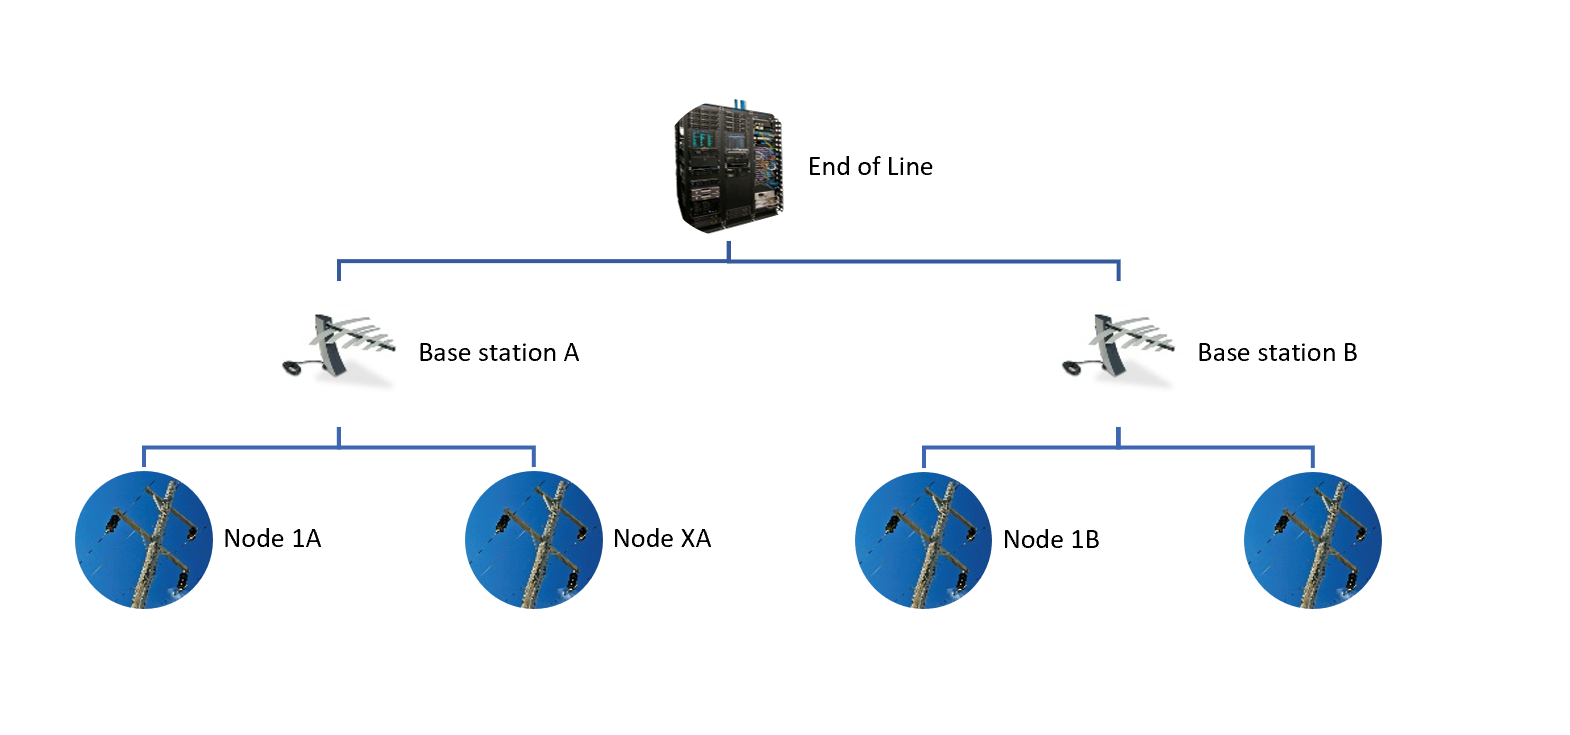
\includegraphics[scale = 1]{Macroscopic system breakdown.PNG}

The node is to send a ‘heartbeat’ signal back to the Base Station when no error is detected by the node. 
If the device detects an error has occurred, it will send a ‘failure’ signal to the Base station. Should 
no signal be received for longer than an acceptable timeframe the system defaults to a ‘failure’ signal 
and thus a team will be dispatched. The base stations are set up along the line of interest each  with  
the ability to contact the End of Line individually. Should a Base Station fail to send the ‘heartbeat’ 
signal it is assumed to be damaged and thus a dispatch is required.

To asses if the pole that the node is connected to is healthy and operating correctly the node will use 
a combination of a digital Accelerometer, Magnetometer and Barometer. This information is then to be 
processed by the Microcontroller within the node. Each node will an independent power supply powered by 
a photovoltaic panel.  This is to reduce dependency on the power lines being monitored.

System Breakdown: \\
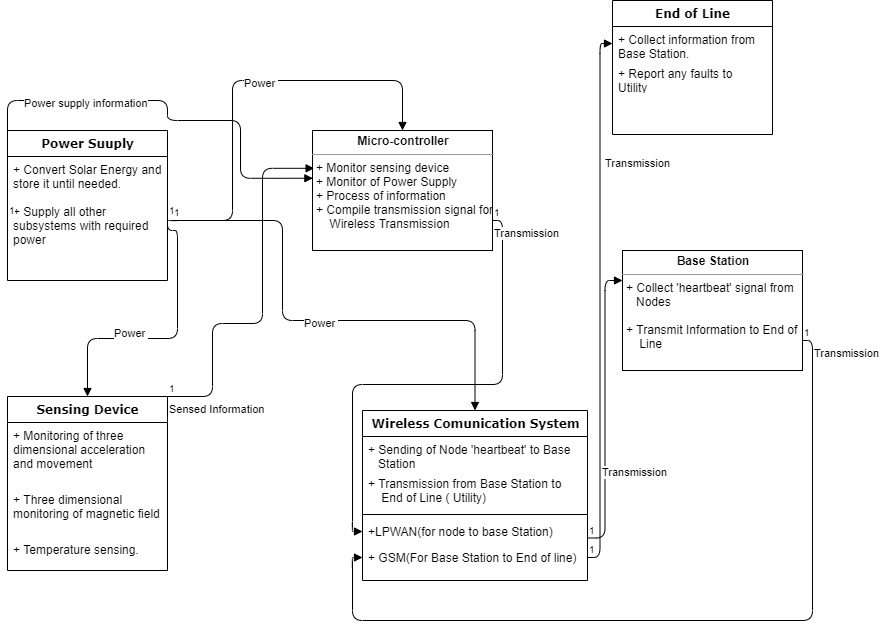
\includegraphics[scale = 0.6]{System Design.jpg}

\section{Sensing Subsystem Design}
\subsection{Device Selection}
Pololu AltIMU-10 v5 is the chosen sensor for this project. There are three integrated circuits embedded on the board that
we will make use of; the LSM6DS33, LIS3MDL and the LP525H. The LSM6DS33 has a gyroscope and accelerometer. 
These are used to track the motion of the pole; tilt, free-fall, orientation change. 
The LIS3MDL has a magnetometer, compass and temperature sensor.
The LP525H has a digital barometer on it to measure pressure. 
We will look at each of the onboard chips to see how they functionalities unite to create this sensing device and the 
features that enable us to use it. 

[https://www.pololu.com/product/2739],[https://www.pololu.com/file/0J1105/altimu-10-v5-dimension-diagram.pdf]
\subsection{Accuracy}
Sensing devices must be able to retrieve information of the pole’s current situation and relay that data to the onboard 
signal receptors accurately, process the data and prepare it for transceival to a responding device. This means the on 
board sensor must be sensitive enough to receive the signal, but not too sensitive to external stimuli that the results 
are altered. The results received must also not stray too far from the expected results.

The AltIMU-10 boasts a high level of accuracy when compared to its v4 predecessor. 
The sensitivity of the device is not affected by temperature or by the passing of a long period of time. 
The output signal generated by this device does not deviate far from the expected ideal output signal either. 
This is because the LSM6DS33 chip has zero-g and zero-rate levels linked to the accelerometer sensors. 
The LIS3MDL has zero-gauss levels linked to its magnetometer sensors. 
This ensures that the results produced are highly accurate. 

Sensing devices also need an accurate reference system. This will enable the device's changes in time to be compared 
with the initial position of the pole. An absolute referencing system is obtained through independent rotation, 
acceleration and magnetic readings to create an altitude and heading reference system. An additional reading from the 
barometer provides an absolute pressure measurement to add to the reference system. 
This will then allow functions such as tilt detection to have an absolute frame of reference. 

The tilt detection function monitors the tilt kinetic acceleration and is based on a trigger event. Should the tilt of 
the device change by an angle greater than 35 degrees from the starting position, then an event is triggered. So should 
the pole’s angular orientation change by an angle of 35 degrees, then so does the angle of the device and an event 
interrupt is sent through.

The LSM6DS33 has various modes of operation. The one chosen for this sensing project is the case when both the gyroscope
and accelerometer are active for continuous monitoring of data from both devices. During active mode, the gyroscope and 

accelerometer must perform at the appropriate frequencies discussed in the modelling subsection . The gyroscope and accelerometer can operate at low power
modes. This is configured by setting G_HM_MODE bit in CTRL7_G (16h) and XL_HM_MODE bit in CTRL6_C (15h) to 1. 

The gyroscope is accurate at tracking rotation on a short time-scale only. In order to compensate for this, the 
accelerometer is coupled with the compass on the LIS3MDL.
The LIS3MDL’s accuracy is affected by high currents which power poles are prone to. High currents affect the magnetic 
field readings which are important for the functioning of the compass. They can alter these readings and cause errors.

[https://www.pololu.com/file/0J1087/LSM6DS33.pdf],[https://www.pololu.com/file/0J1089/LIS3MDL.pdf]
\subsection{Device Interfacing}
The three ICs in this instance are selected as the slave devices. The microcontroller they are embedded onto uses the 
I2C serial protocol and SPI communication protocol to communicate with the chips. We will use the I2C protocol. 
The Vin of the microcontroller is connected to a 2.5V to 5.5V power source. Vdd is connected to a 3.3V source.
All GND terminals are connected to the same ground. The I2C has a clock line and data line denoted by SCL and SDA 
respectively. When either of them are high, the voltage is set to Vin for these terminals and when they are low, they 
are set to GND. 

Communication with the chips is facilitated through the I2C interface. 
The I2C protocol is responsible for reading and writing from and to the registers of the chips. 
The I2C bus carries 2 signals; the clock signal (SCL) and the data line signal (SDA). The 3 ICs are the designated slave
devices which are addressed by the master. The board is the master device which generates the clock signal, addresses 
the slaves and can initiate or halt the transfer of data.

The master device generates a clock signal and sends it through the SCL line to the ICs connected on the I2C bus. The SCL
line is then high. The master device also generates a data line signal causing the SDA pin to transition from a low to a
high. This transition from a low to a high data line while the clock signal is high initialises the start condition. 
The master device then sends a byte of data to all ICs. The first seven bits of the byte specify the address of the 
chip. A device to write to and/or read from is selected by specifying the address of the IC. 

[https://www.pololu.com/file/0J1090/LIS3MDL-AN4602.pdf]
\begin{table}[]
  \begin{tabular}{|l|l|}
    \hline
  IC       & IC Address (SAD) \\\hline
  LSM6DS33 & 110101xb         \\\hline
  LIS3MDL  & 00111x0b         \\\hline
  LP525H   & 101110xb        \\ \hline
  \end{tabular}
\end{table}
The SDO/SA0 pin controls the seventh bits of LSM6DS33 and LP525H and the sixth bit of LIS3MDL. When the pin is set to 1,
it is connected to the supply voltage and when it is set to 0, it is connected to ground. This allows 2 different 
inertial modules to connect to the same chip. In our instance, because each pole has a device, there will be a 1-to-1
connection between an IMU and its internal LSM6DS33 chip. So we will set these bits to 0. The least significant bit of 
the byte is the read or write bit. If the bit is 1 (read mode) the chip will transmit data to the master. If the bit is 
set to 0, the master will write to the registers of the chip. 
When all the ICs have compared the address bits post the start condition and a match is found, the channel for 
communication will open between that IC and the master. The slave device must then transmit a slave acknowledge pulse 
(SAK) to confirm the request for open communication through the data line. 
Another byte of data is transmitted to the IC containing a sub-address (SUB). The SUB is then incremented using the
CNTRL3\_C(12h)(IF\_INC) configuration. The generation of an acknowledge pulse must occur after each byte of data is
transmitted.

If the data line is full, the IC holds the clock line, SCL goes low. The IC does not receive the address and does not
send through an acknowledge pulse to the master. The data line transitions to a high. A transition from low to high of 
the SDA line while the clock line is high initialises the stop condition and the termination of data transfer. 

A temperature sensor is embedded on the magnetometer. It is configured using \\ TEMP\_EN bit in CTRL\_REG1 (20h) and 
is set to "1". 

[https://www.pololu.com/file/0J761/LPS25H.pdf]

\subsection{Modeling of Single axis Vibration}
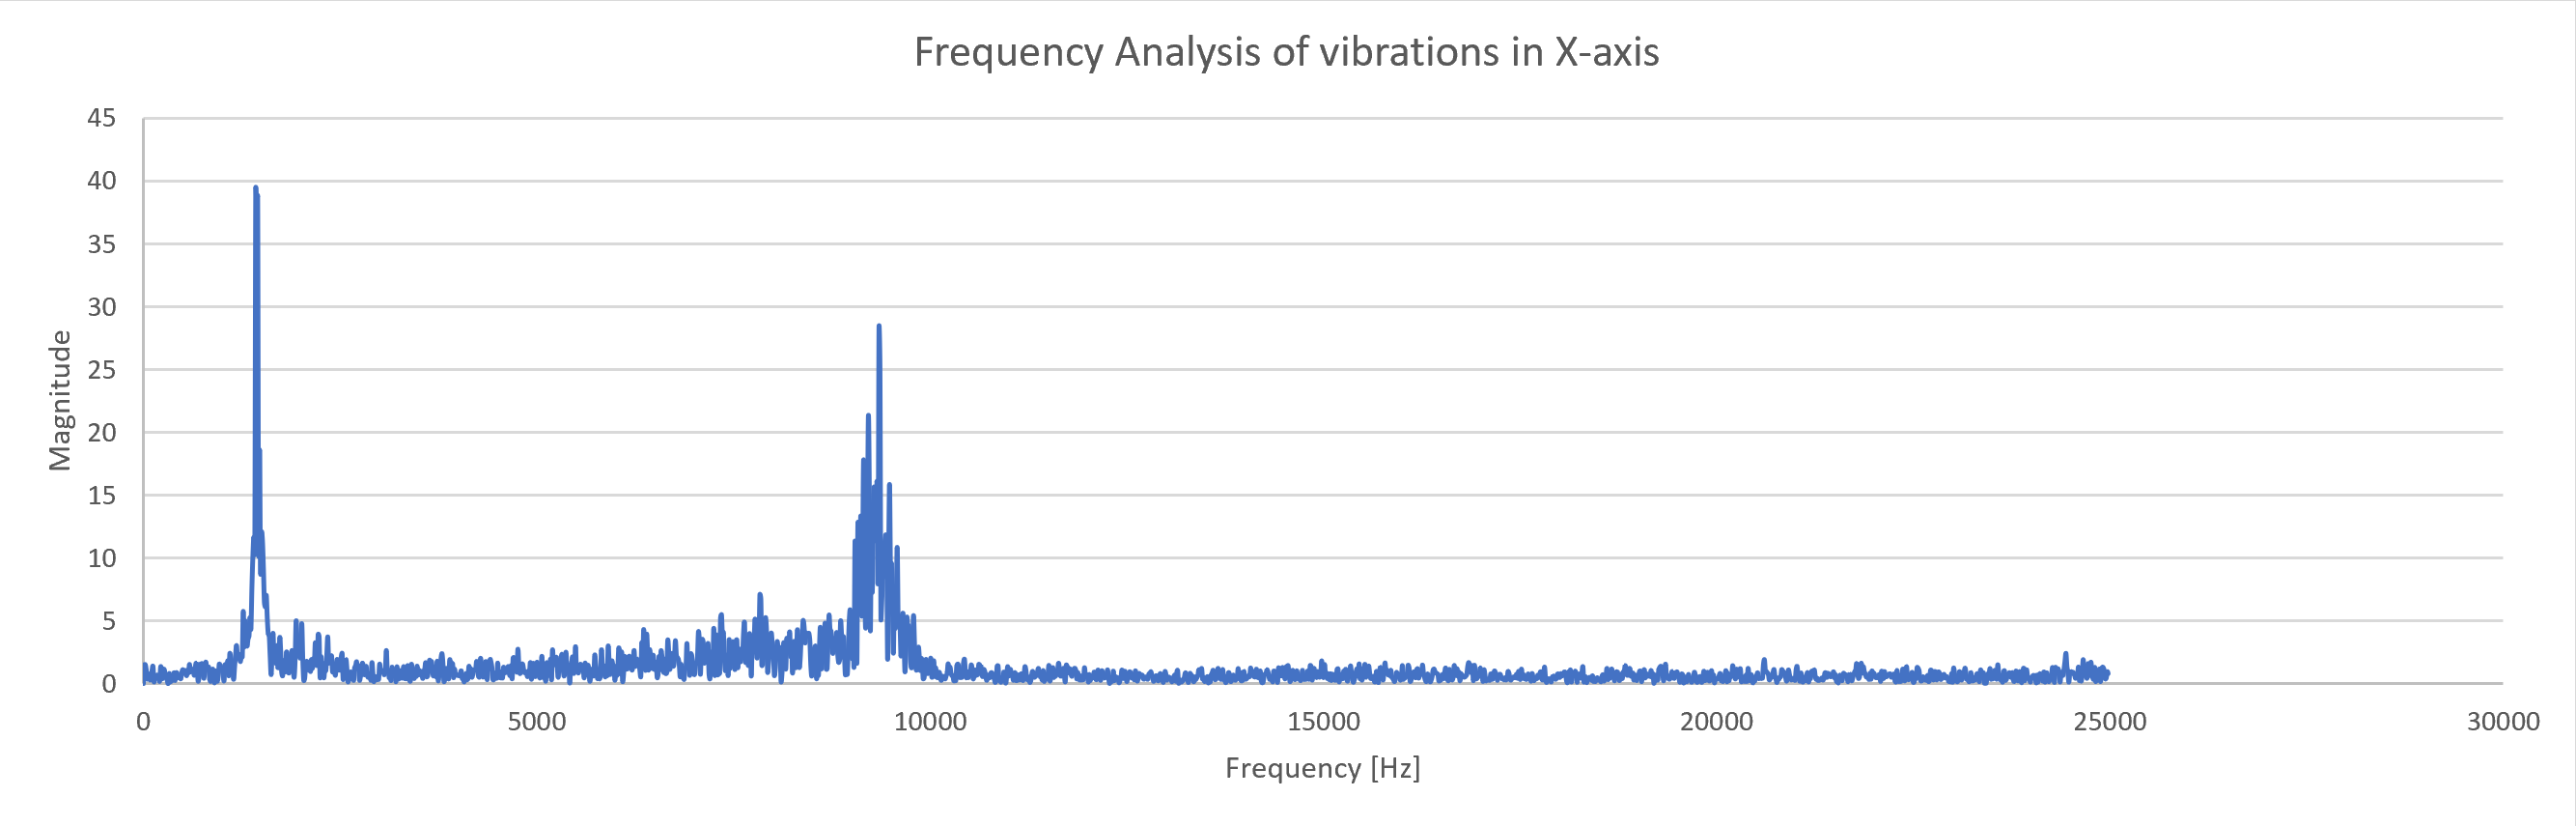
\includegraphics[scale = 0.5]{XaxisVibrations.PNG} 
\\The figure above shows the frequency spectrum of sampled motion on  a single axis. 
The nature of this frequency response is dependent on the physical properties of the pole should any changes, 
gradual (e.i. Rot) or sudden (e.i. Motor car accident), the nature of this frequency response would be affected. 
By comparing these frequency spectrum, physical changes in the pole can be detected. 
In this example we can see that the highest frequency of significance is lower than 10kHz. 
Thus by using Nyquist Sampling Theory to completely sample this signal a minimum sampling rate of 20kHz is required. 

\textit{ The measurements used for generating this model were provided in the 
"Pole measurement data EEE3088.xlsx" File provided by the customer}
\subsection[]{Modeling of Magnetic field from Line Currents}
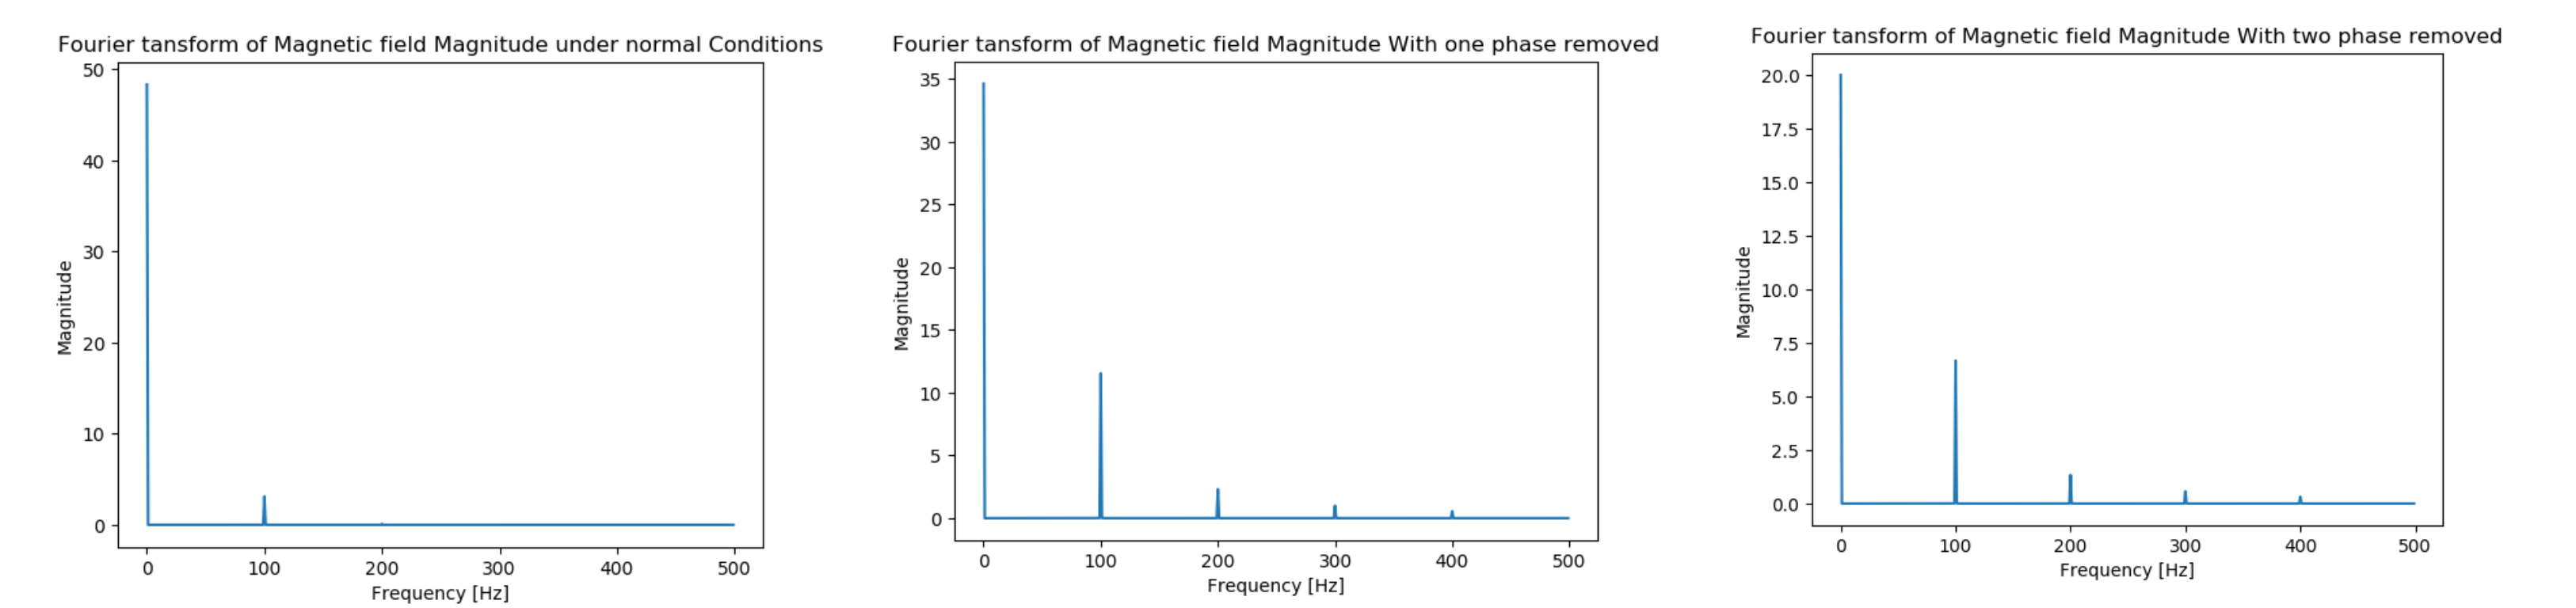
\includegraphics[scale = 0.45]{MagneticFFT.PNG}

The foregoing figures demonstrate how the magnetometer can be used for monitoring of the 3 current carrying lines. 
By making use of just the magnitude of the sensed magnetic field and a Fast Fourier Transform function the device can 
sense the physical displacement of any of the 3 phases. Should one or more of the phases be displaced there is increased
presence of Harmonics. These can be detected at relatively low sampling rates ( minimum 1kHz in this model) reducing the
power draw needed by the device. 
\\ 
\\
With the use of the models presented, this device provides comprehensive error detection of the pole and the 
current-carrying wires without drawing excessive power from the power supply requirements or demanding too much 
computation and data channels  from  the Microcontroller. 

\section{Microcontroller Subsystem Design}

\section{Wireless Communications Design}

\subsection{Wireless Protocol}

The Weightless wireless technology standard has been selected for the wireless communication needs of the wireless commmunications module on the sensor node. Weightless supports supports secure bidirectional data transmission over long distances and is a standard designed for low-power wide area networks (LPWAN) involving base stations and end or terminal devices. For the purposes of the project, some criteria was identified to measure the performance of the wireless technology standard selected: the power efficiency, range, network capacity and  functionality and ease of configurability(complexity) Weightless is a open standard and operates across the range of Industrial, Scientific and Medical ISM, sub GHz  frequency bands for ease of development of IoT systems. 

It was also recognised that interference and noise in urban areas compared to rural areas differ, therefore the transmission range would also be affected in different ways. That's why a wireless standard with an adaptive data rate and transmission power was selected to cater for the different signal paths and the environments in which the base stations and sensors nodes will be placed. That together with the fact that the end devices using Weightless can also be configured to be idle/turn to sleep mode, will allow for better power efficiency and aid to maximise the lifespan of our sensor nodes. 
To also save on costs we also identified the need for a standard that has large network capacity, allowing the use of fewer base stations that can each cover communication between multiple sensor nodes.

%REFERENCES%
%1 . [https://www.ubiik.com/post/2016/09/21/what-is-weightless-p], %
%2 .[https://www.electronicdesign.com/industrial-automation/article/21807028/choosing-the-right-wireless-protocol-for-your-iot-application],%
%3.  [https://radiobridge.com/blog/choosing-the-right-wireless-standard-for-your-iot-sensors]%

\subsection{Message Packet Design}
%Include explanation of FEC%
Weightless uses a radio frame, which acts as a framework, structuring how uplink and downlink data transmission will take place between the end devices and the base stations. This radio frame structure describes the format and access methods for the data packets (MAC layer) and also a physical (PHY layer) description of how the bits of binary data will be formatted into a form suitable for radio transmission. The frame structure is shown in Figure 1:\newline

\begin{figure}[h]
\caption{Frame structure, [1]}
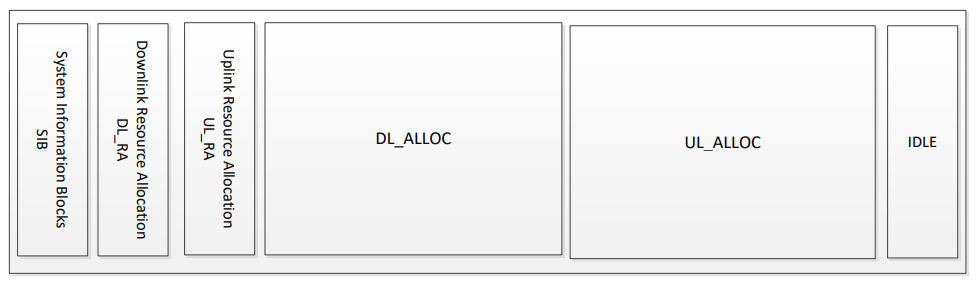
\includegraphics[scale = 0.55]{./images/comms_frame.png}
\end{figure}

Key:
\begin{itemize}
\item SIB: System Information Blocks, used for frame synchronization and to broadcast semi-static parameters of the Base Station and Base Station Network
\item DL\_RA: Downlink Resource Allocation, composed of multiple bursts describing the allocated downlink transmission slots.
\item UL\_RA: Uplink Resource Allocation composed of multiple bursts describing the allocated uplink transmission slots.
\item DL\_ALLOC: the section for allocated downlink transmissions.
\item UL\_ALLOC: the section for allocated and contended uplink transmissions.
\item IDLE: an idle slot in which no End Device is allowed to transmit. Reserved for measurements and future use. [1]
\end{itemize}

It is within this frame structure that the message packet structures for both uplink and downlink transmission are defined, in the  DL\_ALLOC and UL\_ALLOC  sub-frames in Figure 1. Due to the different transmission environments that the sensor modules will be exposed to, careful consideration was taken to ensure that the effects of noise and interference are mitigated to avoid data corruption, which causes errors in the bits of data that are transmitted between the nodes and the base stations. The Weightless standard ensures that the message packets have some form of error correction technique or redundancy. Both the uplink and downlink data packets have the same basic structure as shown in Figure 2: \newline \newline \newline \newline \newline

\begin{figure}[h]
\caption{Message structure, [1]}
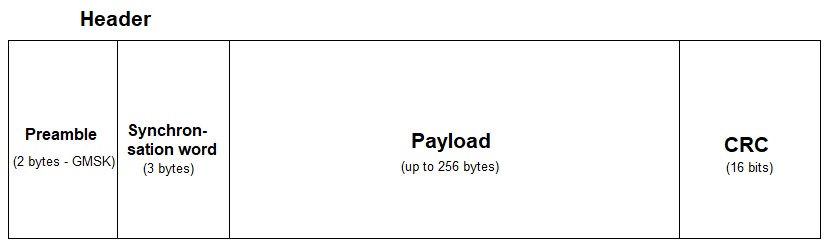
\includegraphics[scale = 0.7]{./images/message_structure.png}
\end{figure}

The header contains contains a preamble which is used to synchronise the communication timing between the base station and end devices and a synchronisation word to indicate, to the end device, the start of data transmission. The header has some form of Cyclic Redundancy Check (CRC), which is an error detection technique that appends a check value ,produced by the transmitter, to the header. This check value is recalculated on the receiver side and compared to the append value to ensure that no errors occurred during transmission.  The payload contains that message intended to be sent between the base station and end device. The payload sub-frame also ends with a CRC with the same error detection purposes, ensuring that the right data is received by the transmitting or receiving device. The data packet can also encoded with a form of error correction, Forward Error Correction (FEC), which can enabled or disabled. FEC is another technique to mitigate the errors that could error during transmission, by encoding the the payload in a redundant way to limit the number of errors and avoid re-transmission of the message.
[1], [2], [3], [4]
%REFERENCES%
%1 . [https://pro-bee-user-content-eu-west-1.s3.amazonaws.com/public/users/Integrators/929cb090-e779-401a-b06c-c629ff6b0fea/ap-cambridgestartuplimi/Weightless-P\_v1.03.pdf], [Undestanding Weightless]%
%2. https://whatis.techtarget.com/definition/preamble%
%3. https://en.wikipedia.org/wiki/Syncword%
%4 .https://en.wikipedia.org/wiki/Cyclic_redundancy_check %
%5. https://en.wikipedia.org/wiki/Forward_error_correction%
\subsection{Range and Error rate simulations}
%Bit Error Rates - Need to find one for  Weightless%
%[https://www.mathworks.com/help/comm/examples/bluetooth-low-energy-bit-error-rate-simulation.html],% 
%[https://www.mathworks.com/help/comm/examples.html?category=rf-propagation]%Range and Power Simulation %

\subsection{Communication Range}

\subsection{Power Consumption}

\subsection{Power Control}

\section{Power Supply Design}
\subsection{User requirements in regards to power supply of system}
The device needs to function 24/7 throughout the year. South Africa is a country with several issues about their power distribution, therefore load shedding would be a major concern when the device is running. This taken in we would use a solar panel and it would charge a battery during daytime. it will have enough energy to supply the device during night time or any other load shedding issues.

The device needs to be easy to maintain throughout the service years and easy to install without requiring too much space. The user would be able to swap batteries and maintain the power supply system for a long period of time.

Since the power supply will be independent from  excess power supplies to maintain the requirement of providing power despite any disruption.

\subsection{Solar energy reliability}
Since the design chose to use a solar-energy system to charge and power the device, for the device to function at its most sufficient power, it relies heavily on the amount of sun light it receives. The main reason the design chooses a solar energy power supply system is because South Africa is one of the best places to use this technology due to its sunny climate. "As Professor Detlev Kröger, Senior Researcher and Emeritus Professor in the Department of Mechanical and Mechatronic Engineering at Stellenbosch University claims that South Africa is one of the best places in the world to develop solar power. "Citing
https://sola.africa/news/south-africas-solar-resource-compared-to-the-rest-of-the-world/


%According to the government website on energy, it states that ``Most areas in South Africa average more than 2 500 hours of sunshine per year, and average solar-radiation levels range between 4.5 and $6.5kWh/m^2$ in one day. " This basically means that the whole country is has sun light most of the time through out the year. "The annual 24-hour global solar radiation average is about 220 W/m2 for South Africa, compared with about 150 W/m2 for parts of the USA, and about 100 W/m2 for Europe and the United Kingdom. This makes South Africa's local resource one of the highest in the world." Citing http://www.energy.gov.za/files/esources/renewables/r_solar.html


Since our device needs to stay alert 24/7 for poles that might fall or short anytime, the power supply needs to be most reliable to the device. The device needs to be on for as long as possible. 

Another main concern was about the duality, and as long as there is sunshine there will be enough energy to supply power towards the system.  

\section{Additional Design Components}

\section{References}
\printbibliography

\section{Appendices}
\subsection{Magnetic field measurement modeling}

This simulation was conducted in Julia programing language with the following code:
\begin{lstlisting}
using PyPlot 
using FFTW

x = 0.4; #dimension of pole [m]
y = 0.3;

# NB! in this simulation the sensor is Modeled as being in the (0,0) position!


μ0 = 1.256637061*10^(-6); #magnetic permeability of air
MagnitudeOfCurrent = 100;  #Estimated average Value of current in wires

Ax = -x;       #defining physical dimensions from sensor to phases
Ay = 0;
Bx= 0;
By = y*99999;
Cx = x*99999999;
Cy = 0;

Ad = sqrt(Ax^2+Ay^2);
Bd = sqrt(Bx^2+By^2);
Cd = sqrt(Cx^2+Cy^2);

t = 0:0.00001: 1;
I_a = MagnitudeOfCurrent*sin.(2*π*t*50);    #current in each of the phases
I_b = MagnitudeOfCurrent*sin.(2*π*50*t.+ (2*π/3));
I_c = MagnitudeOfCurrent*sin.(2*π*50*t .+ (4*π/3));

figure()
plot(t, I_a,t,I_b,t,I_c),
title("Plot of current through all the phases"),
legend(["I_a", "I_b","I_c"])

B(I,d) = μ0*(I)./d    #equation for calculating magnetic
                      # flux from current carrying wire

B_a = B(I_a,Ad);
B_b = B(I_b,Bd);
B_c = B(I_c,Cd);




Btot_y= -B_a + B_c;   #assuming the sensor is at positon (0,0)
                      #these phases only act in the Y direction
Btot_x = B_b    ;    #assuming the sensor is at positon (0,0) 
figure()             #this phase only acts in the X direction
plot(t,Btot_y)

figure()
plot(Btot_x,t)


Bmag = sqrt.(Btot_y.^2+Btot_x.^2);  #calculation of The
                                    # toatal magnitude measured

figure()
plot(t,Bmag)

X = fft(Bmag);


figure()
plot(abs.(X[1:500]))
figure()
plot(abs.(X[1:500])); 
title("Fourier tansform of Magnetic field Magnitude With two phase removed"); 
xlabel("Frequency [Hz]"); ylabel("Magnitude")


\end{lstlisting}



\end{document}